\section{Introduction}

\IEEEPARstart{F}{ollowing} a planned trajectory on a robot while
compensating execution errors has been extensively studied in the 90's
for mobile robots \cite{91icra.samson,
  98deLucaOrioloSamson}. Surprisingly, this issue has not been
explicitly addressed in the literature concerning navigation for
legged robots, although these machines are also prone to execution
errors while moving.

Previous experiments such as \cite{11humanoids.baudouin} illustrate
how imprecise can be trajectory following on a humanoid robot. After
executing a five meters long trajectory, the difference between the
planned and real position can reach $0.4 \textrm{m}$. Such an error
cannot be ignored anymore and invalidate the whole planning
stage. Therefore, solving this issue is crucial and will allow the
achievement of complex movements where a high precision is needed. For
instance, obstacle crossing is only feasible at the beginning of the
trajectory where the drift is not too important. This paper objective
is to provide a generic framework for robust trajectory following on a
humanoid robot.

One way of indirectly tackling the problem consists of regularly
replanning the motion of the robot from its current configuration to
the goal after localizing obstacles with respect to the robot. This
strategy enables the robot to be reactive to environment changes as
well as to execution errors~\cite{05humanoids.michel,
  06icra.MichelChestnut,10springer.chestnut}. On the other hand, it
requires short planning time and induces heavy CPU load. It might even
not be always be possible. Indeed most fast replanning schemes rely on
a simplified model~\cite{01icra.KajitaKanehiro} of the robot
neglecting momenta generated by the leg motions. These assumptions are
not met for small robots like Nao~\cite{wikipedia.nao} with a large
ratio of mass distributed in the legs and with a small CPU.

Moreover, to produce a really feasible movement, additional
constraints must be satisfied: no auto-collision should occur during
the movement for instance.


\begin{figure}[ht!]
  \begin{center}
    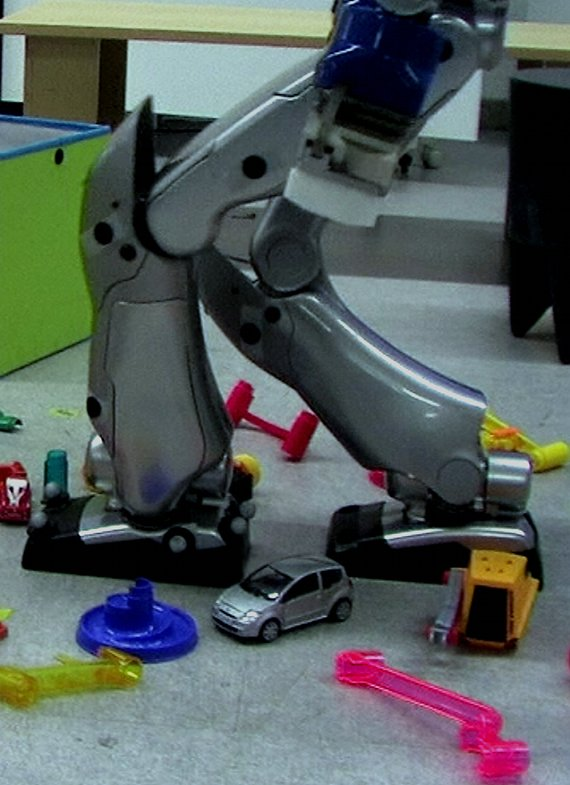
\includegraphics[width=.4\textwidth]{fig/exp2.jpg}
  \end{center}
% 4cm in x and y
  \caption{HRP-2 robot walking in a constrained
    environment. Compensating for execution errors is crucial in this
    scenario to avoid collisions. \label{fig:following}}
\end{figure}



Due to all these factors, validating a complex movement remains a
computationally expensive operation. Therefore, an alternative
solution to online replanning and regeneration of the walking
trajectory such as \cite{11icra.dimitrov, 10ar.herdt,
  06icra.nishiwaki, 05humanoids.michel} is the continuous deformation
of walking trajectories.  This combination of dynamic trajectories and
high probability for the robot to enter in auto-collision makes naive
correction algorithm fail which is why it is important to define a
sound framework for trajectory following.


This paper presents a ``blink of an eye'' reshaping of the trajectory
associated with a generic method to follow trajectories on a humanoid
robot. These two features together provide a way to follow a
trajectory while compensating for errors during the movement
execution. This opens many possible applications such as moving in
extremely constrained environments in a reliable manner, going to
specific places of the environment precisely, etc. Most of the state
of the art demonstration of reactive pattern generators are, in fact,
open loop trajectories with no sensors feedback. This work has been
fully integrated into the LAAS/JRL planning and control frameworks and
a motion capture system has been used to close the loop and evaluate
the execution errors.

This allowed HRP-2 humanoid robot to perform precise and/or long
locomotion tasks where usual open loops approaches would have drifted
so much that the task would have failed.


\section{Motivation}


This work has been motivated by the previous experimental setup
described in \cite{11humanoids.baudouin}. In this paper, fast online
replanning is used to handle environment changes. Using replanning to
cancel the drift has been considered at first but suffers from several
drawbacks. The initial idea was to accelerate replanning and consider
that there is no need to take into account the execution errors as it
can be handled by changing the robot starting position to the position
given by the localization system and regenerate the part of the
trajectory which is yet to be executed. This is difficult in practice
for several reasons. First, using the localization system as an input
of the planning component is dangerous. If the localization is
imprecise, so will be the plan. Therefore, it is required to filter
the robot position explicitly to ensure a high quality localization at
every point of time. On the opposite, as our control scheme only
modifies the next step and is bounded by a correction limit, a
low-pass filter is implicitly applied and protects the control scheme
from temporary erroneous localization. Second, if the localization is
imprecise and is near an obstacle, the estimated position may be in
collision with the obstacle. It is possible to project the robot
position outside the obstacle but additional efforts are required
during the motion planning step. To finish, even if fast replanning is
possible, randomized planning such as RRT-based methods cannot be used
safely in a real-time context as they cannot guarantee to compute a
solution within in a determined time frame. In
\cite{11humanoids.baudouin}, when a replanning is required, the three
next steps cannot be modified to avoid discontinuities in the robot
trajectory. It means that the correction cannot be as reactive as it
may be necessary: the execution error may be taken into account too
late. On the opposite, the next section will demonstrate that
real-time correction is possible.


\begin{figure}[ht!]
  \begin{center}
    \begin{tabular}{|c|c|c|}
      \hline
      \bf{Strategy} & Replanning & Correction\\
      \hline
      \bf{CPU usage}          & High     & Low (real-time)\\
      \bf{Reactivity}         & Low      & High\\
      \bf{Position filtering} & Explicit & Implicit\\
      \hline
    \end{tabular}
  \end{center}
  \caption{Comparison of replanning and online correction when
    compensating for execution errors. \label{fig:comparison}}
\end{figure}



\FloatBarrier

%%% Local Variables:
%%% ispell-local-dictionary: "american"
%%% LocalWords:
%%% End:
